\documentclass[10pt,border=1pt]{standalone}
\usepackage[T1]{fontenc}
\usepackage{mathpazo}
\usepackage{amsmath,amssymb}
\usepackage{xcolor}
\usepackage{pgfplots}
\pgfplotsset{compat=1.18}
\usetikzlibrary{shapes.geometric,positioning,arrows.meta,calc}
\definecolor{okorange}{HTML}{E69F00}
\definecolor{oksky}{HTML}{56B4E9}
\definecolor{okgreen}{HTML}{009E73}
\definecolor{okblue}{HTML}{0072B2}
\definecolor{okverm}{HTML}{D55E00}
\definecolor{okpurple}{HTML}{CC79A7}
\colorlet{accent}{okverm}
\pgfplotsset{
  safenest/.style={
    tick label style={font=\footnotesize},
    label style={font=\small},
    title style={font=\small, align=left},
    legend style={font=\footnotesize, draw=none, fill=none, cells={anchor=west}},
    grid style={black!12, line width=0.3pt},
    axis line style={black!70, line width=0.4pt},
    tick style={black!70, line width=0.4pt},
    axis lines*=left,
  },
}
\newlength{\figwidth}
\tikzset{every node/.append style={execute at begin node={\hyphenpenalty=10000\exhyphenpenalty=10000\relax}}}
\setlength{\figwidth}{18.47cm}
\begin{document}
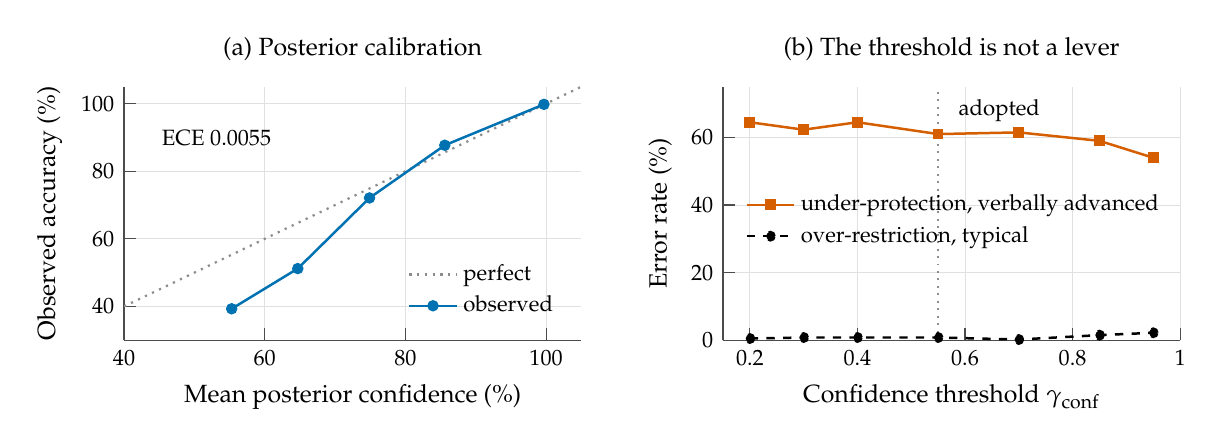
\begin{tikzpicture}
\begin{axis}[safenest, name=l, width=0.40\figwidth, height=48mm,
  xmin=40, xmax=105, ymin=30, ymax=105,
  xlabel={Mean posterior confidence (\%)}, ylabel={Observed accuracy (\%)},
  xmajorgrids, ymajorgrids, title={(a) Posterior calibration},
  legend style={at={(0.97,0.05)}, anchor=south east},
]
\addplot[black!45, dotted, line width=0.8pt] coordinates {(40,40) (105,105)};
\addlegendentry{perfect}
\addplot[mark=*, mark size=1.6pt, okblue, line width=0.9pt] coordinates {(55.3,39.3) (64.7,51.2) (74.9,72.1) (85.6,87.7) (99.7,99.8)};
\addlegendentry{observed}
\node[font=\footnotesize, anchor=west] at (axis cs:44,90) {ECE 0.0055};
\end{axis}
\begin{axis}[safenest, at={($(l.east)+(18mm,0)$)}, anchor=west,
  width=0.40\figwidth, height=48mm, xmin=0.15, xmax=1.0, ymin=0, ymax=75,
  xlabel={Confidence threshold $\gamma_{\mathrm{conf}}$}, ylabel={Error rate (\%)},
  xmajorgrids, ymajorgrids, title={(b) The threshold is not a lever},
  legend style={at={(0.03,0.62)}, anchor=north west},
]
\addplot[mark=square*, mark size=1.5pt, accent, line width=0.9pt] coordinates {(0.2,64.5) (0.3,62.3) (0.4,64.5) (0.55,61.0) (0.7,61.5) (0.85,59.0) (0.95,54.0)};
\addlegendentry{under-protection, verbally advanced}
\addplot[mark=*, mark size=1.5pt, black, dashed, line width=0.9pt] coordinates {(0.2,0.5) (0.3,0.8) (0.4,0.8) (0.55,0.8) (0.7,0.2) (0.85,1.5) (0.95,2.2)};
\addlegendentry{over-restriction, typical}
\draw[black!45, dotted, line width=0.7pt] (axis cs:0.55,0) -- (axis cs:0.55,75);
\node[font=\footnotesize, anchor=west] at (axis cs:0.57,68) {adopted};
\end{axis}
\end{tikzpicture}
\end{document}
